\subsection{Dobbeltensretter}
\label{Dobbeltensretter}
%
Dobbeltensretterens formål er at eliminere negative analoge spændinger fra differensforstærkeren, ved at invertere negative spændinger til positive spændinger, hvorfor det kun er amplitudens fortegn der ændres for negative spændinger og de positive spændinger bibeholdes. Grunden til at der implementeres en dobbeltensretter i kredsløbet er fordi A/D konverteren kun kan håndtere positive analoge inputsignaler. I situationer hvor outputspændingen fra volumenkontrollen er mindre end outputspændingen fra referencen vil outputtet fra differensforstærkeren være negativt og så vil A/D konverteren sende forkerte bits videre til multiplekserne, og det vil derfor ikke være muligt at sikre at det er de korrekte filtre der vælges. 

På \autoref{fig:DobbeltensretterXY} illustreres princippet bag en dobbeltensretter, hvor de negative amplituder af et analogt inputsignal inverteres til positive amplituder, samtidig med at de i forvejen positive amplituder bibeholdes. Så uafhængigt af fortegnet på outputtet fra differensforstærkeren, så vil dobbeltensretteren altid sørger for dens eget output er positivt. 
%
\begin{figure}[H]
	\centering
	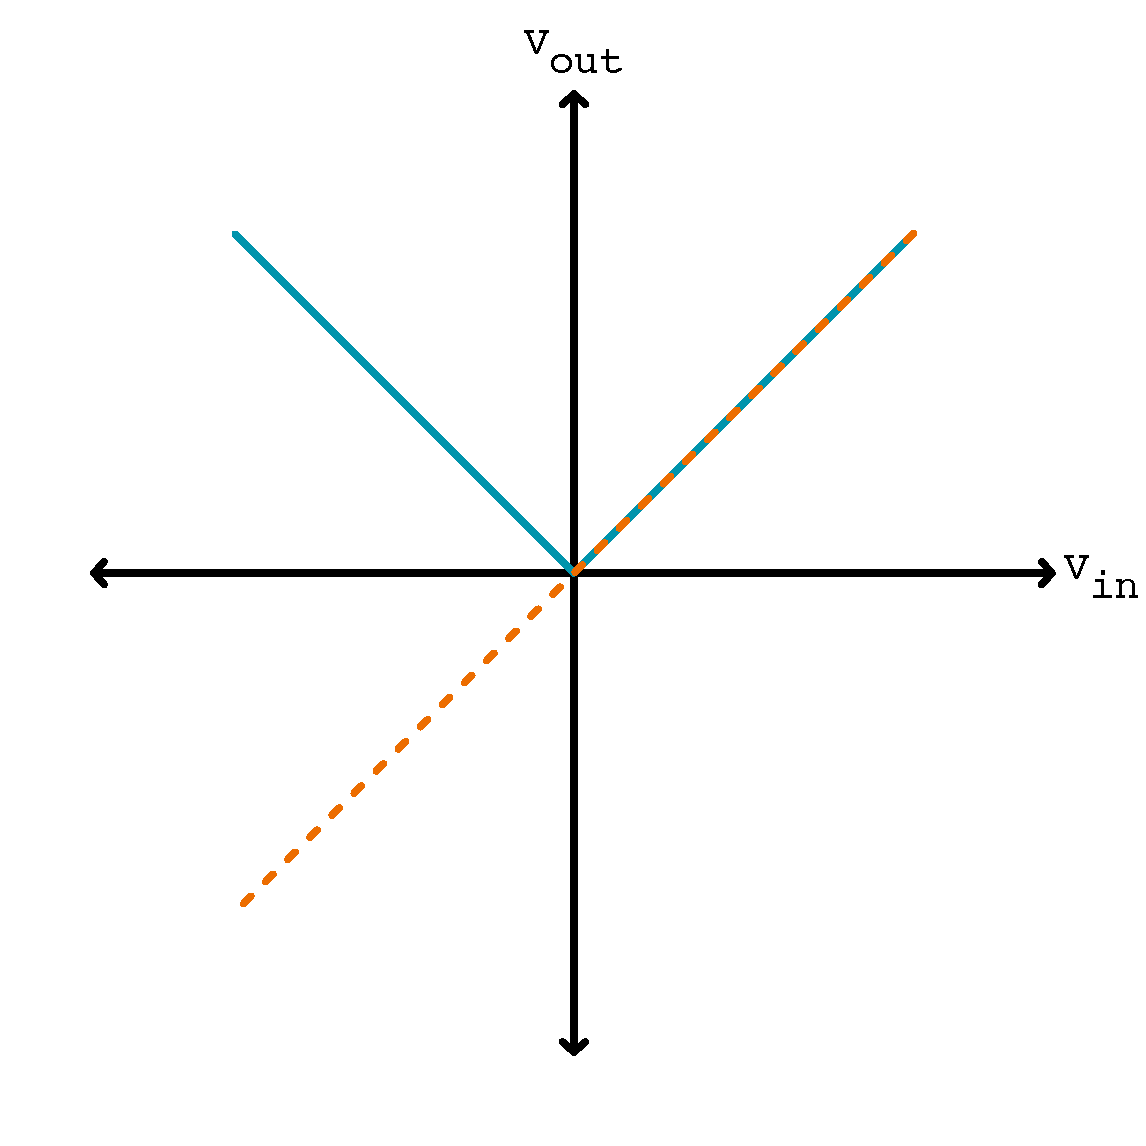
\includegraphics[resolution=300,scale=\circuitSize]{Figure/Circuits/DobbeltensretterXY.pdf}
	\caption{En tilnærmelsesvis ideel overføringskarakteristik for en dobbeltensretter. Hvor x-aksen angiver inputspændingen, $V_{in}$, y-aksen angiver outputspændingen, $V_{out}$, den stiplede orange linje er inputtet og de blå kontinuerlige linjer er outputtet.}
	\label{fig:DobbeltensretterXY}
\end{figure}
\noindent
%
Når outputtet fra differensforstærkeren er 0, vil forholdet mellem $V_{in}$ og $V_{out}$ være i origo (0,0), hvorfor de lave frekvenser ikke modificeres. Det første kvadrant på \autoref{fig:DobbeltensretterXY} repræsenterer tilfælde hvor outputspændingen fra volumenkontrollen overskrider referencens outputspænding, svarende til at differensforstærkeren giver et positivt output. Det tredje kvadrant repræsenterer tilfælde hvor outputspændingen fra volumenkontrollen er mindre end outputspændingen fra referencen, svarende til at differensforstærkeren giver et negativt output. Når det er tilfældet vil dobbeltensretteren invertere det negative signal fra trejde til andet kvadrant, jævnfør \autoref{fig:DobbeltensretterXY}. 
%
\begin{figure}[H]
	\centering
	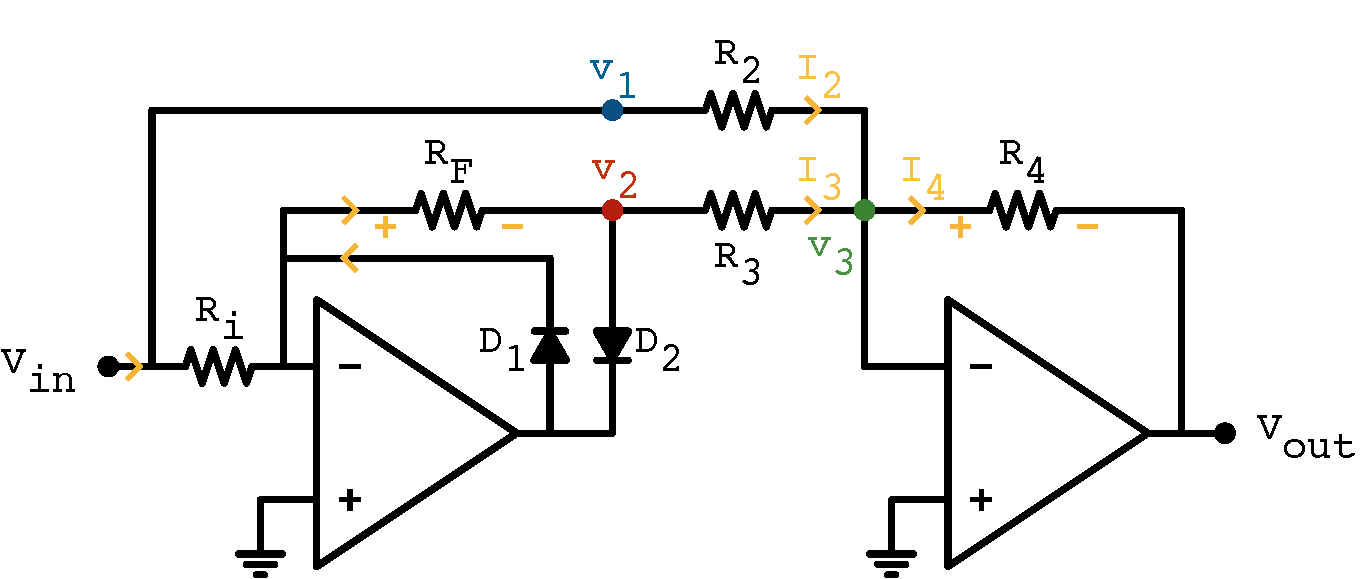
\includegraphics[resolution=300,scale=\circuitSize]{Figure/Circuits/Dobbeltensretter.pdf}
	\caption{Kredsløbsdiagram for opkoblingen af en dobbeltensretter, som består af en enkeltensretter, koblingen på den første operationsforstærker, efterfulgt af en inverterende adder, koblingen på den anden operationsforstærker.}
	\label{fig:Dobbeltensretter}
\end{figure}
\noindent
%
Hvis inputtet er positivt, $V_{in} > 0$, vil outputtet fra den første operationsforstærker være negativt, derfor vil $D_2$ være forspændt i lederetningen, hvilket medfører at der løber strøm igennem dioden, og $D_1$ vil være forspændt i spærreretningen, som medfører at der ingen strøm kan løbe igennem dioden. I dette tilfælde vil den anden operationsforstærker fungere som en inverterende summationskobling, som derfor inverterer det negative signal til et positivt outputsignal, $V_{out}$. Hvorimod hvis inputtet, $V_{in}$, er negativt så er outputtet fra den første operationsforstærker positivt, og $D_2$ vil være forspændt i spærreretningen og $D_1$ være forspændt i lederetningen. Grundet virtuel jord så er outputtet fra enkeltensretteren 0, hvilket medfører at outputtet, $V_{out}$, bliver positivt. 

De to dioder, afbilledet på \autoref{fig:Dobbeltensretter} er af typen BAT85, \parencite{PDF:Diode}. Diodernes opgave er at sørge for at strømmen kun kan løbe den ene vej, fra anoden (+) til katoden (-). Generelt er dioder meget følsomme overfor temperaturændringer, men for at minimere diodernes følsomhed og for at undgå mætning kobles de i en tilbagekobling med operationsforstærkeren. Ved at placere dioderne i tilbagekoblingen fjernes spændingsfaldet over dioderne, og fordi signalet bliver taget ud fra $R_3$ og ført videre i kredsløbet, så er det muligt at se bort fra diodespændingen, hvorfor dioderne fungere som ideelle dioder.
%
\begin{figure}[H]
	\centering
	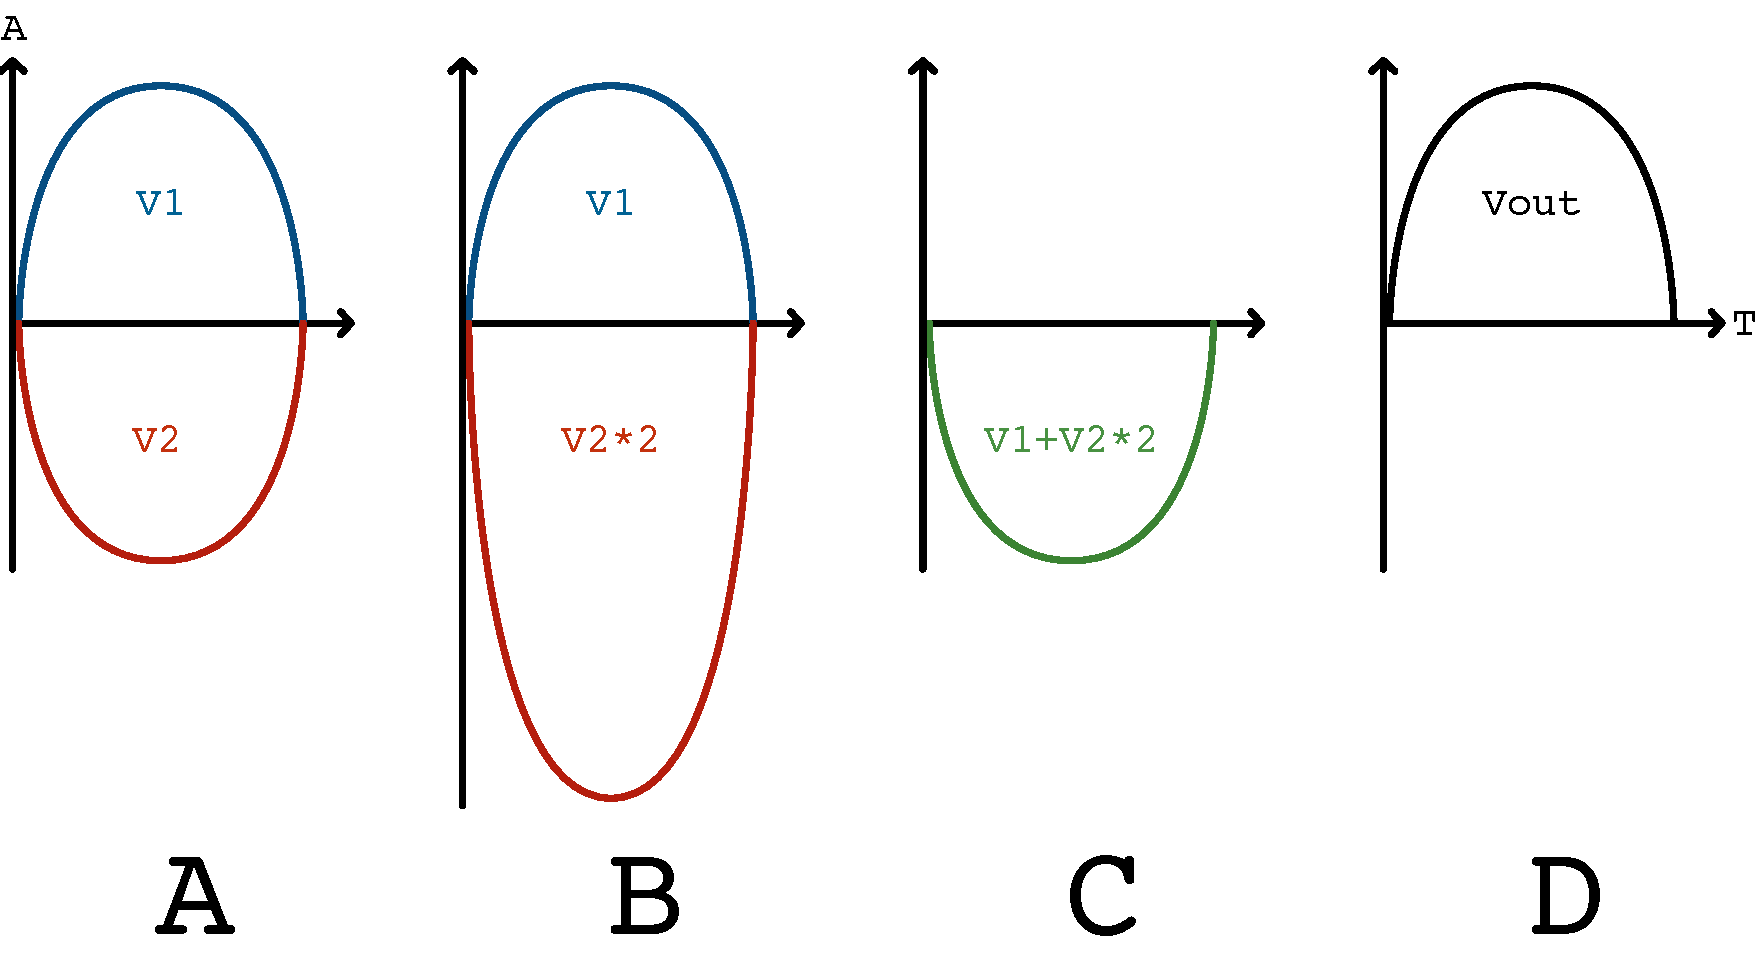
\includegraphics[resolution=300,scale=\circuitSize]{Figure/Circuits/Dobbeltensretter_SignalForloeb_Positive.pdf}
	\caption{Signal forløbet igennem dobbeltensretteren, såfremt $V_{in}$ er positiv.}
	\label{fig:Dobbeltensretter_SignalForloebPos}
\end{figure}
\noindent
%
På \autoref{fig:Dobbeltensretter_SignalForloebPos} illustreres signal forløbet  for et positivt signal på $V_{in}$, hvor \autoref{fig:Dobbeltensretter_SignalForloebPos}A gengiver hvordan inputsignalet fremstår i noderne: $v_1$ og $v_2$. I node $v_1$ er signalet uændret fordi det ikke føres igennem enkeltensretteren, hvor i node $v_2$ er signalet blevet inverteret af enkeltensretteren. På \autoref{fig:Dobbeltensretter_SignalForloebPos}B, som er forløbet lige efter signalet har passeret henholdvist $R_2$ og $R_3$, fremgår signalet uændret efter $R_2$, hvor det fordobles efter at have passeret $R_3$. Fordoblingen sker fordi modstanden af $R_3$ er halvt så stor, som de resterende modstande. Inden signalet inverteres af den inverterende adder, så adderes signalerne, der er illustreret på \autoref{fig:Dobbeltensretter_SignalForloebPos}B, hvilket resulterer i signalet illustreret på \autoref{fig:Dobbeltensretter_SignalForloebPos}C. Den inverterende adder sørger derefter for at signalet inverteres og bliver positivt, hvilket fremgår af \autoref{fig:Dobbeltensretter_SignalForloebPos}D. 
% 
Med udgangspunkt i \autoref{Dobbeltensretter} og \autoref{fig:Dobbeltensretter_SignalForloebPos} er det muligt, at udlede følgende overføringsfunktioner, for et positivt inputsignal. Først udledes overføringsfunktionen for når signalet er i knudepunktet $v_2$, som angiver at det før positive signal, nu er inverteret hvorfor $V_{in}$ har et negativt fortegn: 
%
\begin{equation}
	V_2 = \frac{-V_{in}*R_F}{R_i}
\end{equation}
%
Grunden til at $v_3 = 0$ skyldes at potentialet på den inverterende adder er 0.
%
\begin{equation}
	v_3 = 0
\end{equation}
%
 Så kan strømmen i knudepunktet $v_3$ beregnes, ved hjælp af Kircchoff's strømlov, som forudsætter at alle strømme ind i et knudepunkt er lige strømmen ud af knudepunktet: 
%
\begin{equation}
	I_4 = I_2+I_3
\end{equation}
%
Så $I_4$ er strømmen igennem $R_4$, derfra er det muligt at udlede overføringsfunktionen for $V_{out}$:
%
\begin{equation}
	V_{out} = -R_4*I_4
\end{equation}
%
Hvis inputtet derimod er negativt, $V_{in} < 0$, så vil signalet blive elimineret af ensretteren, men fordi inputsignalet også bliver ført udenom dobbeltensretteren fra $V_{in}$ og fordi der ikke forekommer et spædningsfald over $R_3$, så sker der kun en addition med 0, hvorfor det negative signal inverteres til et positivt output på $V_{out}$. 
%
\begin{figure}[H]
	\centering
	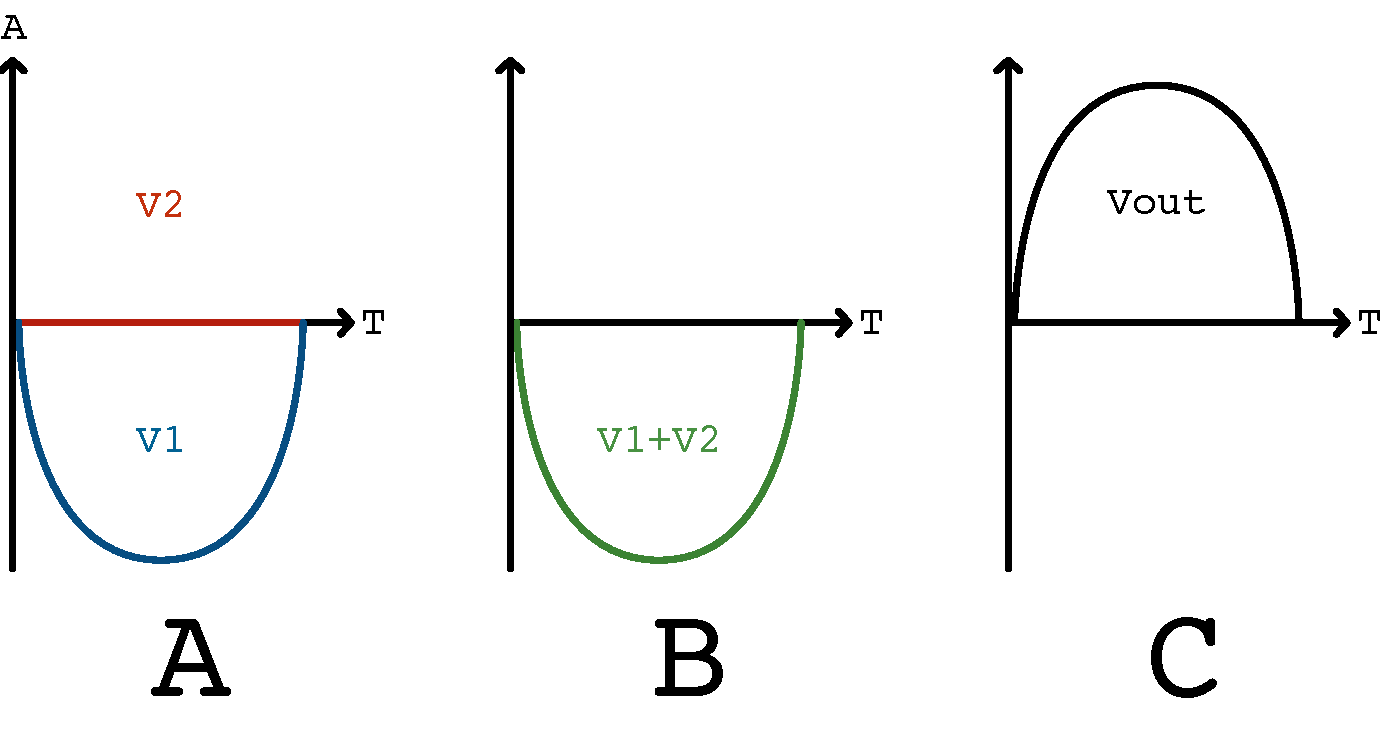
\includegraphics[resolution=300,scale=\circuitSize]{Figure/Circuits/Dobbeltensretter_SignalForloeb_Negative.pdf}
	\caption{Signal forløbet igennem dobbeltensretteren, såfremt $V_{in}$ er negativ.}
	\label{fig:Dobbeltensretter_SignalForloebNeg}
\end{figure}
\noindent
%
På \autoref{fig:Dobbeltensretter_SignalForloebNeg} illustreres signal forløbet  for et negativt signal på $V_{in}$, hvor \autoref{fig:Dobbeltensretter_SignalForloebNeg}A gengiver hvordan inputsignalet fremstår i noderne: $v_1$ og $v_2$. I node $v_1$ er signalet uændret da det ikke føres igennem enkeltensretteren, hvorimod i node $v_2$ er signalet elimineret af enkeltensretteren. Ligesom ved tilfældet med et positivt inputsignal adderes de to noder, hvilket repræsenteres på \autoref{fig:Dobbeltensretter_SignalForloebNeg}B. Det negative inputsignal bliver derefter inverteret af den inverterende adder, og resultatet deraf er $V_{out}$ og gengives på \autoref{fig:Dobbeltensretter_SignalForloebNeg}C.

Følgende overføringsfunktion udledes, såfremt inputsignalet på $V_{in}$ er negativt: 
%
\begin{equation}
	V_{out} =  \frac{-V_{in}*R_4}{R_2}
\end{equation}
%
At overføringsfunktionen kun indeholder $R_2$ og $R_4$, skyldes at inputsignalet elimineres af enkeltensretteren, så ved kundepunktet $v_3$ bliver det negative signal adderet med 0, hvorefter det inverteres af den inverterende adder. At $R_4$ har et negativt fortegn skyldes at modstanden sidder i tilbagekoblingen. 
%  
\begin{figure}[H]
	\centering
	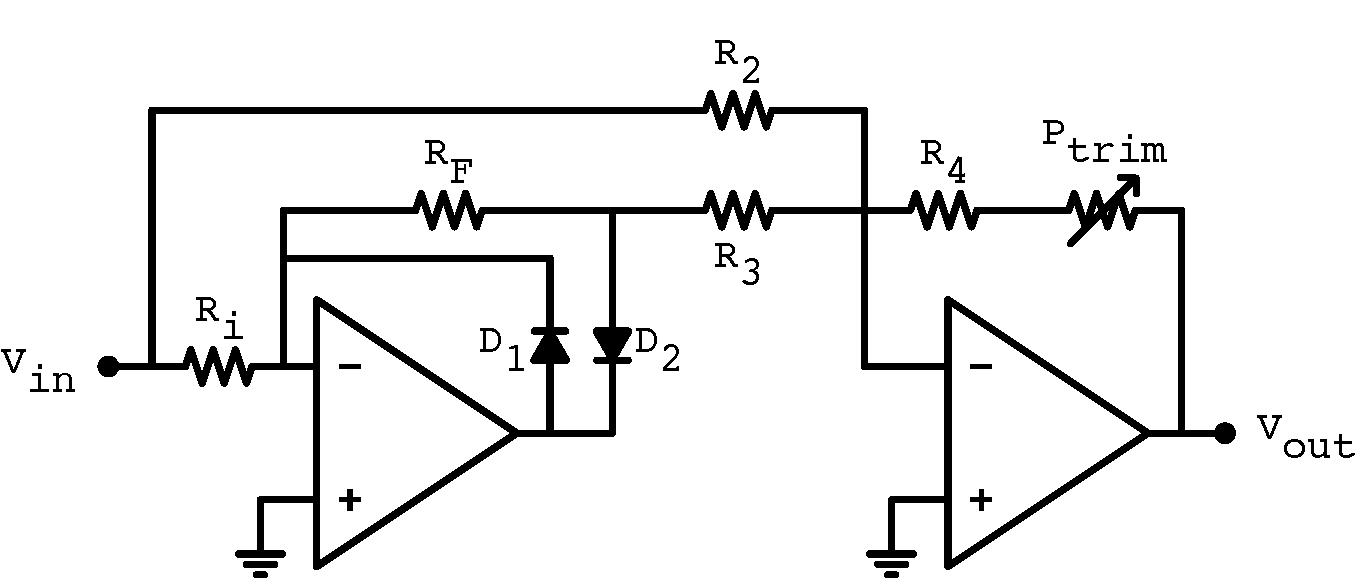
\includegraphics[resolution=300,scale=\circuitSize]{Figure/Circuits/Dobbeltensretter_Trim.pdf}
	\caption{Kredsløbsdiagram for opkoblingen af den anvendte dobbeltensretter.}
	\label{fig:Dobbeltensretter_Trim}
\end{figure}
\noindent
%
I den endelige opkobling tilføjes der et trimmepotentiometer, $P_{trim}$ i serie med tilbagekoblingsmodstanden på den inverterende adder, jævnfør \autoref{fig:Dobbeltensretter_Trim}. Trimmepotentiometeret har til formål at forstærke $V_{out}$, så når A/D konverteren modtaget outputtet fra dobbeltensretteren så vil det være forstærket til en maksimal spænding på 4.3V. Grunden til at signalet skal forstærkes skyldes at A/D konverteren fungerer mere stabilt ved en højere spænding. Spændingen A/D konverteren modtager skal makismalt have samme værdi, som den positive forsyningsspænding, $+V_F$, på +5V, hvilket ligeledes svarer til den spænding differensforstærkeren maksimalt modtager på de to input terminaler. Såfremt trimmepotentiometeret ikke inkluderes ville A/D konverteren maksimalt kunne modtage en inputspænding på +2V.\\[5mm]
%
Der er brugt to operationsforstærkere i dobbeltensretteren, som tilhører den samme IC, TL074, som differensforstærkeren. Hvor operationsforstærkeren til enkeltensretteren får inputspændingen på den inverterende terminal, ben 2, den ikke-inverterende terminal, ben 3, er i jord og outputtet kobles til ben 1. Operationsforstærkeren til den inverterende adder får ligeledes en inputspænding på den inverterende terminal, på ben 13, den ikke-inverterende terminal, ben 12, er i jord og outputtet fra dobbeltensretteren, $V_{out}$, kobles til ben 14.

Fire ud af de fem modstande i dobbeltensretteren, angivet på \autoref{fig:Dobbeltensretter}, har den samme værdi:
%
\begin{equation}
	R_i = R_F = R_2 = R_4 = 10k\Omega
\end{equation}
%
Hvor $R_3$ angives til at være halvdelen af denne værdi, så $R_3 = 5k\Omega$ og $P_{trim}$ er på $12k\Omega$.


